% Please add the following required packages to your document preamble:
% \usepackage{multirow}
%\label{change}


%Schema changes include addition, deletion, renaming on table, column, association, index, and constraint, and type change on association and column. For example, a column could change from a `int' type to a `string' type. And an association could change from `has\_one' to `has\_many'.  

\textbf{Extended motivation.}
A recent study~\cite{wang2017verifying} on 100 Rails applications 
%with more than 400 commits 
showed that most applications went through many schema changes.
%are common: about 28 per application on average.
%database schema has been changed at least once in all these 100 applications, with the average 
%about 28 schema changes on average over each application's life time.  
For further motivation, we studied
12 Rails and Django web applications from different categories like forum, e-commerce, social network, etc. \footnote{The application list is in our code
repository.} They are all highly rated, each with
more than 1000 stars on GitHub, 11,000--900,000 lines of code and 500--100,000 commits. 


% Schema change could happen on table, columns, associations, and indices
% % \junwen{Isil's group also shows constraints change, we didn't since it's covered in previous paper and will not cause query issue}; 
% a change could be addition, deletion, renaming. Besides, for column and association, it also contains type change. For example, a column could change from a `int' type to a `string' type. And an association could change from `has\_one' to `has\_many'. 
% \begin{table}[]
\caption{Application Corpus}
\label{tab:apps}
\resizebox{1\columnwidth}{!}{
\begin{tabular}{llrrrr}
\hline
\hline
Name & Category & \# stars & \# commits & \# versions & \# loc \\
\hline
Lobsters & Forum & 3k & 2.1k & 19 & 11 k \\
Gitlab & Collaboration & 22.6k & 100k & 1040 & 932k \\
Spree & E-commerce & 11.3k & 23.4k & 244 & 74k \\
Tracks & Management & 1k & 4.4k & 19 & 16k \\
Diaspora & Social Network & 12.7k & 20k & 82 & 83k \\
Onebody & Social Network & 1.4k & 5.2k & 32 & 103k \\
\hline
Zulip &  Collaboration & 13.7k  & 42.5k & 78 & 162k \\
Awx & Management & 9.7k & 29.7k & 45 & 93k \\
Saleor & E-commerce & 11.1k & 18.5k & 142 & 174k \\
Healthchecks & Management & 3.8k & 1.7k & 26 & 17k \\
Gerapy & Management  & 2.4k & 0.5k & 26 & 22k \\
Posthog &  Collaboration & 4.1k & 3.1k & 52 & 39k \\
\hline
\hline
\end{tabular}
}
\end{table}

\textit{How often are schema changes?} 18\% -- 85\% of application versions
contain at least one schema change, and there are more than 8 changes for every
version on average.
Furthermore, changes are common throughout the development history of each
application. For example, across the 6 Rails applications, the most recent 25\%
of commits happen to contain about 25\% of all the schema
changes in total.

%, as shown in Table~\ref{tab:change-stat}.
%Note that, for all  applications except for Lobsters \cite{lobsters}, we treat every public code release as a version; since Lobsters does not specify code release/version, we treat every 100 code commits as one version. 

\textit{What types of changes are there?} As shown in Table \ref{tab:change-stat},
 changes to various aspects of the schema
 %tables, columns, association relationships (e.g., `has\_one'
%or `has\_many' relationship between two tables), and table indices, 
are all common.
About three quarters of changes add tables, columns, or indices, and
do not directly cause inconsistency with existing code. The remaining
one quarter of changes modify or delete existing tables, columns,
associations, or indices, immediately threatening code consistency, and hence
are the target of \ETool, as detailed
in Table \ref{tab:overview}.


\iffalse 
\textbf{How schema changes vary with age?} We split every application' history into four quarters, each with the same number of releases/versions and count the average number of schema changes in each quarter (time gaps between code releases
are stable within each application). As shown in Figure~\ref{fig:evo-time}, although there are more changes in the first two quarters, changes in the latter two quarters
are still common.
%, indicating that schema-related refactoring is necessary for applications at any development stage no matter it's new or mature. 
%\shan{If you want to save space, you can replace Figure 1 with a text explanation saying how many changes are there in each major version: I assume there are 13 major versions for AWX? Based on AWX, I feel there are indeed more schema changes at the beginning, but there are still a good amount of changes lat j er on. That is probably a more fair claim.}


\begin{figure}
    \centering
    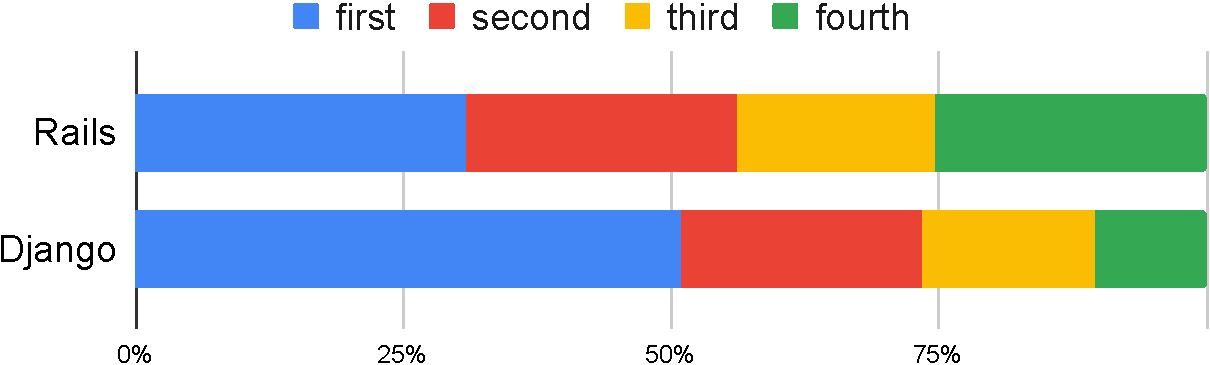
\includegraphics[width=\columnwidth]{figs/breakdown-4.pdf}
    \caption{Quarter Breakdown of Schema Changes (Aggregated View)}
    \label{fig:evo-time}
\end{figure}
% \shan{Explain how is your study different from that by
% Isil's group. It is also fine if your study is similar
% with Isil's group's study, and just that you look at different sets of applications. No matter what is the case, please explain clearly.}
\fi 


% \shan{need to introduce these applications a bit. why you choose these applications to study; how large they are; how long they have been under development, etc.}

%Overall, schema changes of various types broadly exist in applications across their development phases. Related refactoring support will be broadly beneficial.






\begin{table}
\caption{Number of Schema Changes per Version}
\label{tab:change-stat}
\centering
%\setlength{\tabcolsep}{2pt} 
%\resizebox{\columnwidth}{!}{
\begin{tabular}{lrrrrr}
\arrayrulecolor{black}\hline  
\arrayrulecolor{black}\hline
Change Target  & Table  & Column  & Association  & Index  & Total \\
\arrayrulecolor{black}\hline
Django & 1.0           & 4.4            & 2.6                & 0.2     & 8.2      \\
Rails  & 1.6           & 4.8            & 2.2                & 1.3  & 9.9     \\   
\arrayrulecolor{black}\hline  
\arrayrulecolor{black}\hline
\end{tabular}
% \begin{tabular}{l|rr}

% \arrayrulecolor{black}\hline  
% \arrayrulecolor{black}\hline
% Types & Django  &  Rails \\ \hline
% Table Changes & 1.1 & 1.6 \\
% Column Changes & 4.7 & 4.8 \\
% Association Change & 2.5 & 2.2 \\
% Index Changes & 0.1 & 1.3 \\ 
% \hline
% Total & 8.4 & 9.8 \\

% \arrayrulecolor{black}\hline  
% \arrayrulecolor{black}\hline
% \end{tabular}
%}
\end{table}




